\documentclass[a4paper,12pt,oneside,final]{report}
%\usepackage{geometry}                % See geometry.pdf to learn the layout options. There are lots.
%\geometry{landscape}                % Activate for for rotated page geometry
%\usepackage[parfill]{parskip}    % Activate to begin paragraphs with an empty line rather than an indent
\usepackage{graphicx}
\usepackage{amssymb}
\usepackage{epstopdf}
\usepackage[utf8]{inputenc}
\usepackage{titlesec}
\titleformat{\chapter}[hang]{\bf\Huge}{\thechapter}{1cm}{}

\pagestyle{plain}
% -------------------- this stuff for code --------------------

\usepackage{anysize}
\marginsize{30mm}{30mm}{20mm}{20mm}

\newenvironment{formal}{%
  \def\FrameCommand{%
    \hspace{1pt}%
    {\color{blue}\vrule width 2pt}%
    {\color{formalshade}\vrule width 4pt}%
    \colorbox{formalshade}%
  }%
  \MakeFramed{\advance\hsize-\width\FrameRestore}%
  \noindent\hspace{-4.55pt}% disable indenting first paragraph
  \begin{adjustwidth}{}{7pt}%
  \vspace{2pt}\vspace{2pt}%
}
{%
  \vspace{2pt}\end{adjustwidth}\endMakeFramed%
}

\newenvironment{changemargin}[2]{\begin{list}{}{%
\setlength{\topsep}{0pt}%
\setlength{\leftmargin}{0pt}%
\setlength{\rightmargin}{0pt}%
\setlength{\listparindent}{\parindent}%
\setlength{\itemindent}{\parindent}%
\setlength{\parsep}{0pt plus 1pt}%
\addtolength{\leftmargin}{#1}%
\addtolength{\rightmargin}{#2}%
}\item }{\end{list}}

\usepackage{color}
\usepackage{dsfont}
\usepackage[bitstream-charter]{mathdesign}
\usepackage[scaled]{helvet}
\usepackage{inconsolata}


\definecolor{colKeys}{rgb}{0,0,0.9} 
\definecolor{colIdentifier}{rgb}{0,0,0} 
\definecolor{colString}{rgb}{0.7,0,0} 
\definecolor{colComments}{rgb}{0,0.6,0} 
\usepackage{listings}
\lstset{
  stringstyle=\color{colString},
  keywordstyle=\color{colKeys},
  identifierstyle=\color{colIdentifier},
  commentstyle=\color{colComments},
  numbers=left,
  tabsize=4,
  frame=single,
  breaklines=true,
  basicstyle=\small\ttfamily,
  numberstyle=\tiny\ttfamily,
  framexleftmargin=0mm,
  xleftmargin=8mm,
  xrightmargin=8mm,
  frameround={tttt},
  captionpos=b
}

%% Headers and footers
\usepackage{fancyhdr}
\usepackage[section]{placeins}
\pagestyle{fancy}
\fancyhf{}
\addtolength{\headwidth}{30pt}
\addtolength{\headwidth}{30pt}
\renewcommand{\headrulewidth}{0.4pt} % thickness of the header line
\renewcommand{\footrulewidth}{0.4pt} % thickness of the footer line
\renewcommand{\chaptermark}[1]{\markboth{#1}{#1}} % chapter name
\renewcommand{\sectionmark}[1]{\markright{\thesection\ #1}}  % section name
\lhead[\fancyplain{}{\bf\thepage}]{\fancyplain{}{\bf\rightmark}} % display header
\rhead[\fancyplain{}{\bf\leftmark}]{\fancyplain{}{}} % display header
\fancyfoot[C]{\bf\thepage} % display footer (page number)
\fancyfoot[R]{\bf\today} % display footer (date)
\fancypagestyle{plain}{ 
	\fancyhead{} \renewcommand{\headrulewidth}{0pt}
}
\newcommand{\clearemptydoublepage}{\newpage{\pagestyle{plain}\cleardoublepage}}

\usepackage[T1]{fontenc}
\usepackage{enumerate}
\usepackage{afterpage,lastpage,fancyhdr}
\usepackage[includeheadfoot,margin=2.5cm]{geometry}
\geometry{letterpaper}                   % ... or a4paper or a5paper or ... 

% -------------------- end of code stuff --------------------



\DeclareGraphicsRule{.tif}{png}{.png}{`convert #1 `dirname #1`/`basename #1 .tif`.png}

%\title{Machine Learning Decision Trees Coursework}
%\author{Jean Kossaifi (jk712, a5) \\Sedef Ozlen (so512, s5) \\Paul Gribelyuk (pg1312, a5) \\Romain Brault (rb812, a5)}
%\date{}                                           % Activate to display a given date or no date

\makeatletter \def\thickhrulefill{\leavevmode \leaders \hrule height 1pt\hfill
\kern \z@} \renewcommand{\maketitle}{
    \begin{titlepage}
    \let\footnotesize\small \let\footnoterule\relax \parindent \z@ \reset@font
    \null\vfil
    \vspace{-20mm}
    \begin{center}
    {\small \scshape Imperial College London}
    \end{center}
    \vspace{0.5cm}
	\begin{minipage}{\textwidth}
		\vspace{1cm}
		%\noindent\rule[0ex]{\textwidth}{4pt} \\
		%\flushright
		\center
		\@title
		\\ \vspace{4mm}
		%\noindent\rule[0ex]{\textwidth}{4pt} \\
	\end{minipage}
	\vspace{2cm}
	\begin{center}
		
\includegraphics[width=70mm,]{logo_imperial_college_london.png}
	\end{center}
	\vspace{5.4cm}
	\vspace{\stretch{1}}
	\begin{minipage}{\textwidth}
		\flushright
		{\bfseries}
		\vspace{7mm}
		\center
		\@author\\
	\end{minipage}
	\vspace{20mm}
		\flushleft
		{\bfseries}
		{\small \scshape \@date }
		\vspace{0.1cm}
		\rule{\linewidth}{.5pt}
  \end{titlepage}
  \setcounter{footnote}{1}
  \setcounter{page}{2}
}


\author{Jean Kossaifi (jk712, a5) \\Sedef Ozlen (so512, s5) \\Paul Gribelyuk (pg1312, a5) \\Romain Brault (rb812, a5)}
\makeatother
\title{\Huge Machine Learning Decision Trees Coursework}
\date{\today}


\begin{document}
\maketitle
\tableofcontents
\listoffigures
\chapter{Building the decision trees}
\paragraph{}
We implemented the decision trees algorithm via modular, object-oriented approach to allow flexibility when testing and modifying the algorithm.  This also allowed us to split the work between the team members and used GitHub for version control.
\paragraph{}
The workhorse class responsible for representing the tree is defined recursively as a node, which has "kids", i.e. child nodes, which, in turn, represent subtrees of the tree.  We store the information gain and the depth of the node in the tree, which we later used in the decision-making algorithm when the tree classifier gave ambiguous results.  The project is split up into the following files:
\begin{itemize}
\item[-] \emph{ID3Driver.m}: This function takes (i) examples, (ii) targets, (iii) attributes (as column indices), (iv) a decision function, (v) and the number of folds to use for validation as inputs, and return the confusion matrix, $F_{\alpha}$, a classification rate, and the six binary trees (as an array of nodes).
\item[-] \emph{ID3.m}: This is the algorithm which learns the binary tree by processing the examples until leaf nodes are reached.
\item[-] \emph{tnode.m}: This is the object representation of a node in a tree.  It can have an arbitrary number of child nodes, as well as properties such as ig (information gain), op (node label), and indop (index into the attribute array that this node has split the data on).
\item[-] \emph{ChooseBestDecisionAttribute.m}: This function returns the attribute that splits the data along the lines of the maximal information gain.
\item[-] \emph{trainer.m}: This method is responsible for producing the 6 trees given a set of examples, attributes, and targets.
\item[-] \emph{binaryFromMultiple.m}: Simple method which takes in target data with multiple classifications and converts it to a binary classification.
\item[-] \emph{classify.m}: Given some trees, example data, and a decision function, this method returns an array of predicted classifications.
\item[-] \emph{igClassify.m}: Our decision function which classifies the example data based on the sum of the information gains down a tree when an ambiguous situation arises (i.e. when either more than one tree returns a positive answer, or when all trees return a negative answer).
\item[-] \emph{depthClassify.m}: Another decision function we devised which resolves ambiguities based on shortest depth in the case of more than one positive answer, and longest depth in the case of all negative answers.
\item[-] \emph{NFoldValidationMask.m}: This is a helper function which returns 2 masks of "count" data points, for training and testing "N" times.
\item[-] \emph{ConfusionMatrix.m}: This method takes in predicted and actual target data and returns a confusion matrix.
\end{itemize}

\section{Tree Diagrams}
\paragraph{}
The six following figures have been obtained after training on the whole clean emotion dataset.

\begin{figure}[!h]
\center
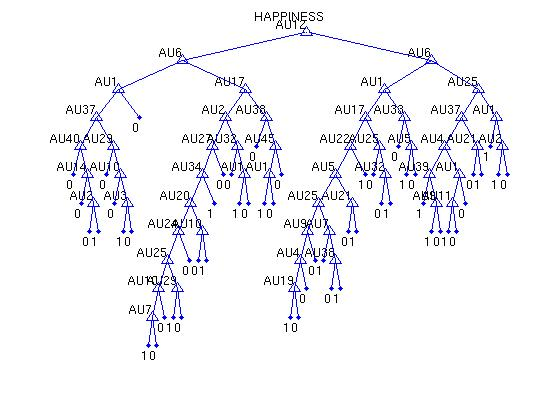
\includegraphics[scale=0.6]{happiness.jpg}
\caption{Happiness Tree.}
\end{figure}

\begin{figure}[h]
\begin{changemargin}{-20mm}{-20mm}
\begin{center}
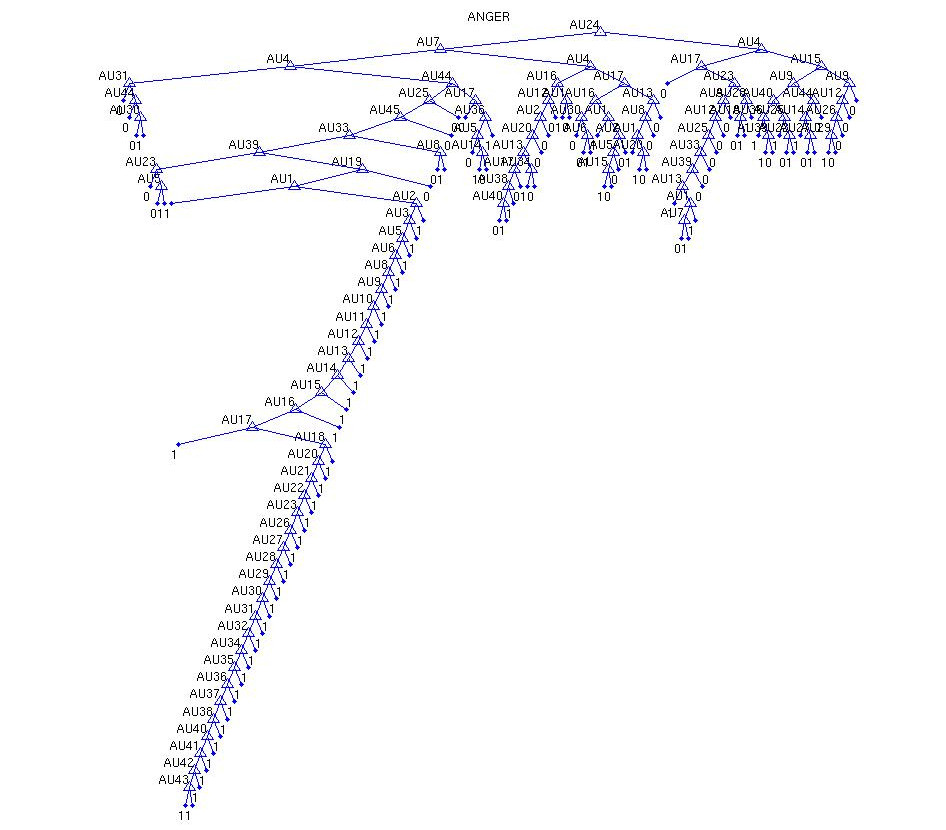
\includegraphics[scale=0.6]{anger.jpg}
\end{center}
\caption{Anger Tree.}
\end{changemargin}
\end{figure}

\begin{figure}[!h]
\center
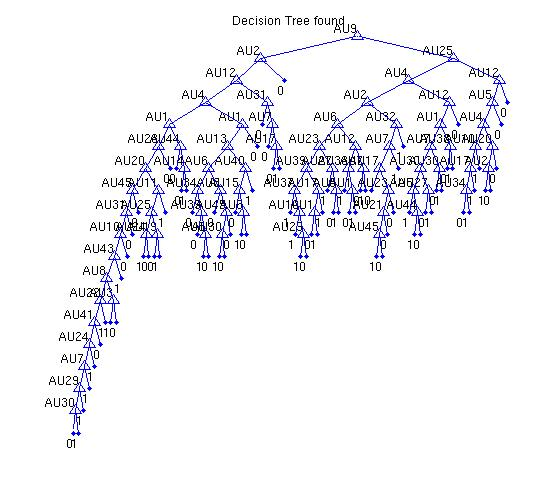
\includegraphics[scale=0.6]{disgust.jpg}
\caption{Disgust Tree.}
\end{figure}

\begin{figure}[!h]
\center
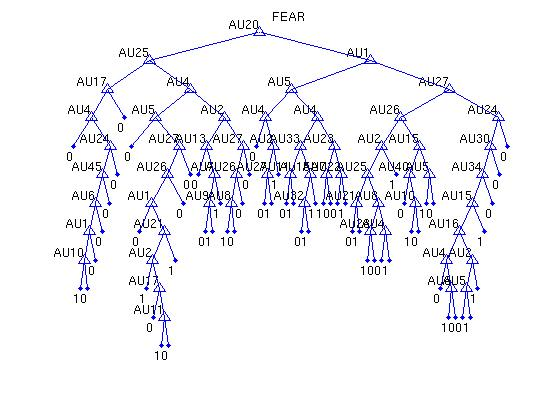
\includegraphics[scale=0.6]{fear.jpg}
\caption{Fear Tree.}
\end{figure}


\begin{figure}[!h]
\center
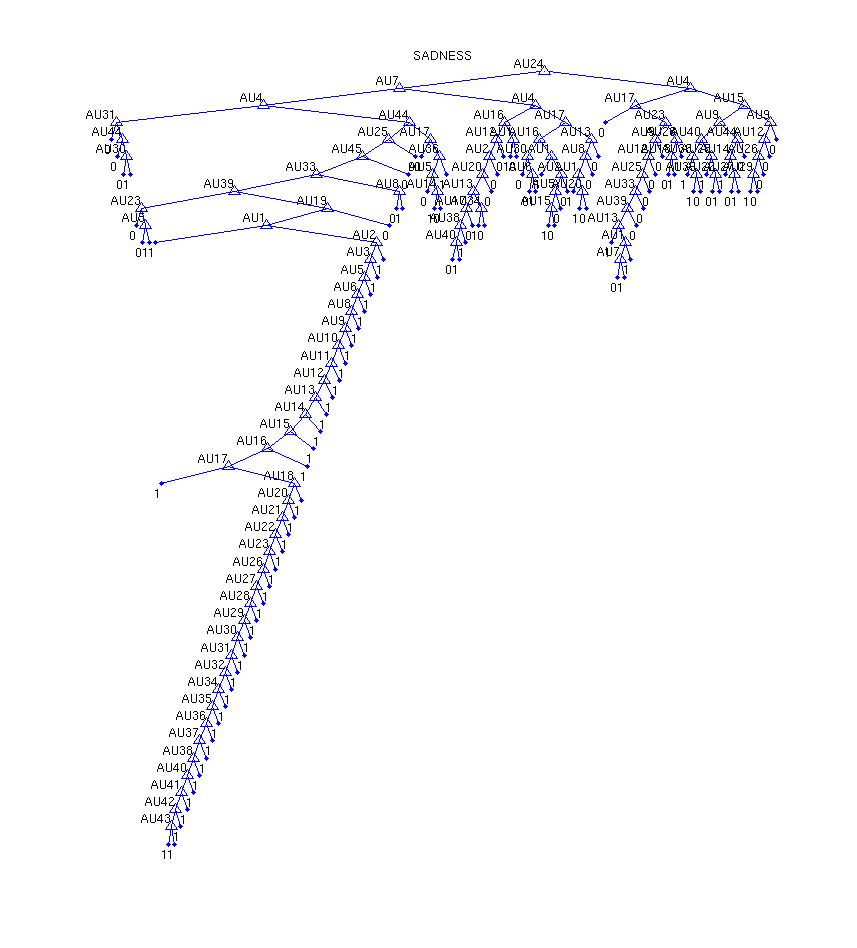
\includegraphics[scale=0.6]{sadness.jpg}
\caption{Sadness Tree.}
\end{figure}

\begin{figure}[!h]
\center
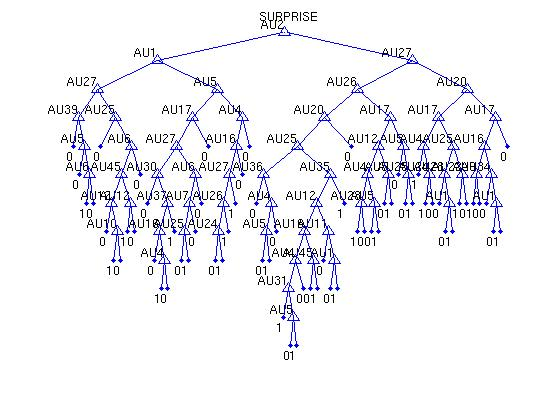
\includegraphics[scale=0.6]{surprise.jpg}
\caption{Surprise Tree.}
\end{figure}
\FloatBarrier

\section{Results}
\paragraph{}
To obtain the results, we run the following code:
\newline
\begin{lstlisting}[language=MATLAB, frame=single]
[cm, err, cr, tr] = ID3Driver(x, 1:45, y, @igClassify, 10);
\end{lstlisting}
\paragraph{}
The confusion matrix received for a random run of the 10-fold cross-validation is as follows(In our implementation of 10-fold cross-validation, we first shuffle the initial array, then divide to folds, hence there may be a difference in values for each run of cross-validation on the same data):
\[
cm = \left[\begin{array}{cccccc}
9.7000   & 9.7000 &   0.5000 &   0.1000 &   1.7000    &0.2000 \\
    1.9000   &15.1000&    0.1000&    0.6000&    1.4000 &   0.6000 \\
    1.2000    &0.7000    &8.4000    &0.2000    &0.5000   & 0.9000 \\
    0.5000    &1.4000    &0.4000   &17.7000   & 0.7000   & 0.8000 \\
    2.6000    &1.4000    &0.6000    &0.6000    &7.6000    &0.3000 \\
    0.2000    &0.5000    &1.8000    &0.6000    &1.0000   &16.5000 \\
\end{array}
\right]
\]
\paragraph{}
The rows of the confusion matrix represent the actual classifications, and the columns represent the predicted classifications for each of the emotions .  They are the average results found by taking the average of all the confusion matrices for each fold of the 10-fold cross-validation process. It seems that our trees have classified most correctly for the 4th emotion, which is happiness. Our average classification rate is   $0.2360$. This rate is found by first summing the times our classifier guessed correctly over the total number of test data for  all 10-folds, and getting the average of it, which gives the correctness percentage. Subtracting this value from 1, gives the error rate. Our classifier can guess over the newly confronted test data with an error rate of approximately $24\%$.  \\
Recall Rates:
\[
recall = \left[\begin{array}{cccccc}
69.6970   &75.7576 &  70.3390  & 88.7850 &  57.2519&   84.0580 \\
\end{array}
\right]
\]
\paragraph{}
Precision Rates:
\[
precision = \left[\begin{array}{cccccc}
71.3178 &   75.7576 &   76.1468 &   85.2018 &   60.0000 &   80.5556  \\
\end{array}
\right]
\]
\paragraph{}
The $F_{\alpha}$ values according to these recall and precision rates are: 
\[
F_{\alpha} = \left[\begin{array}{cccccc}
70.4981 &   75.7576 &   73.1278 &   86.9565 &   58.5938 &    82.2695 \\
\end{array}
\right]
\]
\paragraph{}
As expected, emotion 4 was the best classified emotion, and we achieved the highest rates for both recall and precision.

\chapter{Resolving Ambiguity of Tree Selection}
\paragraph{}
The ambiguity about deciding which binary decision tree to use arises whenever more than one tree returns a positive result or when all trees return a negative result (otherwise, the unique tree which returns a positive classification can be used to make the overall classification).  We first decided to handle these cases based on the aggregate information gain accumulated (additively) when walking down the tree in search of the result.  Our reasoning was that the tree which most clearly divides the data (and thus has the highest cumulative information gain) is more likely to be classifying the emotion.  This turned out to have a better effect than randomly selecting a tree (we obtained $F_{\alpha} \approx 70\%$ and $classError \approx 27\%$ via this method ($F_{\alpha} \approx 75\%$ and $classError \approx 22\%$).  
\paragraph{}
Our second approach was to resolve the ambiguity by selecting the shortest path which gave a positive result among all positive results.  If two paths are of the same length, then the selection resorts to a random one.  If no trees return a positive result, then we select the one which took the longest to traverse to our "no" answer.  Our rationale for this is that we can have the most confidence in the shortest path (which yielded a negative classification), those the longest one should result in the most error-prone answer, thus a "no" is more likely to be a "yes".  We believe that the longer path of a tree is likely the result of noise or overfitting, thus we ascribe less confidence to its prediction.
\paragraph{}
One of the advantages of the depth-based classification decision is that we can avoid the extra overhead of storing data at each node in each tree while we are building it.  However, we believe that the information gain approach produces better results because the maximal information gain could help produce the correct result even when there is some noise further down the tree.  For example, if happiness is described by AU12, AU6, and AU25, then an addition of another action unit to the example could produce a false negative in the answer, but the information gain could be large because the first three action units are very common to the happiness class.  Overall, we believe these approaches work in a similar way, but the information gain has more predictive power.

\chapter{Analysis of Tree Pruning}
\paragraph{}
The \textit{pruning\_example} function start by training a classification tree with the function \textit{treefit} on the dataset thanks to a predictor vector X and a response vector Y. Then the tree is tested with \textit{treetest} by measuring error in two different ways :
\begin{itemize}
\item with a 10 folds cross-validation. Eventually \textit{treetest} return a vector of Cost corresponding to the cross-validation error along the optimal pruning sequence for the tree. It also returns a vector containing the number of terminal nodes of the tree for each cost, and the best level of pruning (eg: the first minimum of the cost vector).
\item With a resubstitution error. Again, the algorithme compute the cost vector along the optimal pruning sequence. The cost for the subtree is the sum over all terminal nodes of the probability to reach the node times the node cost, the node cost being the sum of all misclassified data\footnote{We set the error to 1 for a misclassified element, 0 otherwise}.
The function is also returning the vector cost, the vector of terminal nodes along the optimal pruning sequence and the best level of pruning.
\end{itemize}
Once the tree has been tested with the two error measures discribed above, two pruned tree are created thanks to the best level of pruning computed.
\paragraph{}
Finally the \textit{pruning\_example} function plot the two costs vectors computed with \textit{treetest} as a function of the number of terminal nodes. Figure \ref{fig:pruning} shows the graphic obtained with \textit{pruning\_example} on the clean emotions database. 
The red curve, representing the resubstitution error, keep decreasing until it reach zero with about 200 terminal nodes. At this stage it means that the classification tree doesn't commit any error on the classification date. On the other hand, the blue curve, corresponding to the cross-validation error, stop decreasing after adding about 25 terminal nodes to the tree. This behaviour is caused by the cross-validation error measure since in a cross validation the tree is trained on a random subset of the whole data (9/10) and tested on the remaining part (1/10). As a result the tree cannot overfit the data and the error remains constant.

\begin{figure}[!h]
\center
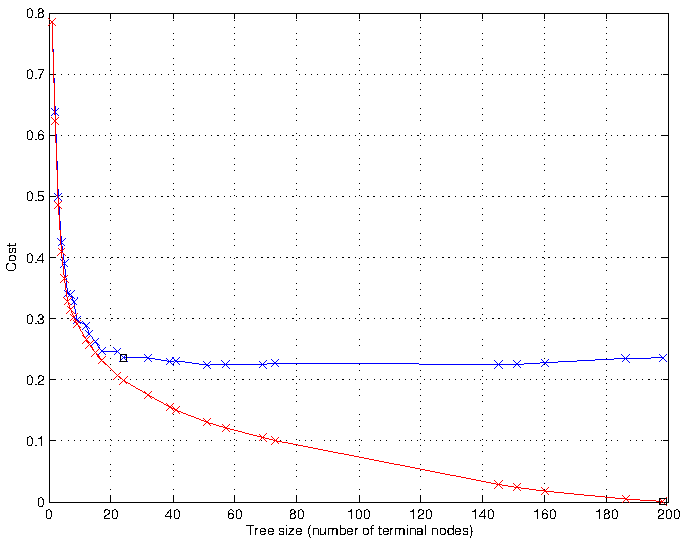
\includegraphics{pruning_example_clean.png}
\caption[Pruning example on clean data.]{Cost computed by cross-validation (blue curve) and resubstitution (red curve) on the clean emotion dataset depending on the number of terminal nodes. \label{fig:pruning}}
\end{figure}
\FloatBarrier
\paragraph{}
Thus the decreasing trend of the red curve while the blue curve slightly increase is a typical indicator of overfitting. The tree is predicting perfecly the training set but is no able to generalise on the test set. It is a good practice to prune the tree or stop learning when the cross-validation error stop decreasing (blue box on figure \ref{fig:pruning}). On the clean data, the cross validation remains constant after 25 terminal nodes. As a result one can belive that it is not dangerous to overfit. However the same study on the noisy dataset (figure \ref{fig:pruning_noisy}) shows that with "real life" data, overfitting can lead to an increase of the cross-validation error.
\begin{figure}[!h]
\center
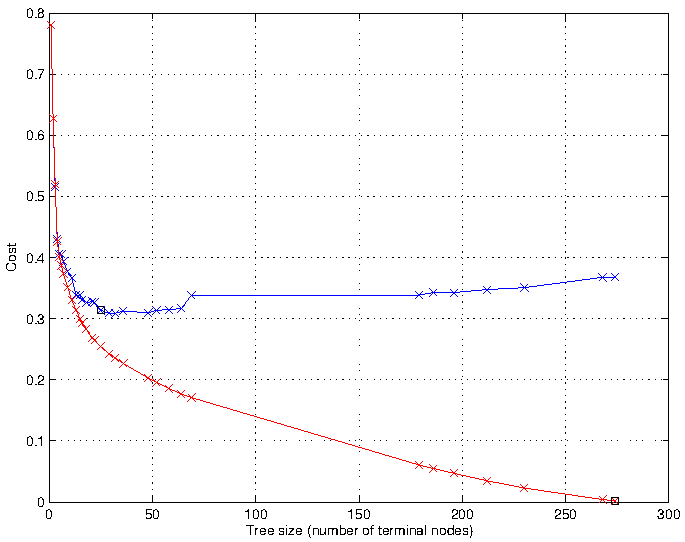
\includegraphics{pruning_example_noisy.png}
\caption[Pruning example on clean data.]{Cost computed by cross-validation (blue curve) and resubstitution (red curve) on the noisy emotion dataset depending on the number of terminal nodes. \label{fig:pruning_noisy}}
\end{figure}
\chapter{Code Flowchart}
%\subsection{}



\end{document}  